%  LaTeX support: latex@mdpi.com 
%  For support, please attach all files needed for compiling as well as the log file, and specify your operating system, LaTeX version, and LaTeX editor.

%=================================================================
\documentclass[journal,article,submit,pdftex,moreauthors]{Definitions/mdpi} 
%\documentclass[preprints,article,submit,pdftex,moreauthors]{Definitions/mdpi} 
% For posting an early version of this manuscript as a preprint, you may use "preprints" as the journal. Changing "submit" to "accept" before posting will remove line numbers.

% Below journals will use APA reference format:
% admsci, aieduc, behavsci, businesses, econometrics, economies, education, ejihpe, famsci, games, humans, ijcs, ijfs, journalmedia, jrfm, languages, psycholint, publications, tourismhosp, youth

% Below journals will use Chicago reference format:
% arts, genealogy, histories, humanities, jintelligence, laws, literature, religions, risks, socsci

%--------------------
% Class Options:
%--------------------
%----------
% journal
%----------
% Choose between the following MDPI journals:
% accountaudit, acoustics, actuators, addictions, adhesives, admsci, adolescents, aerobiology, aerospace, agriculture, agriengineering, agrochemicals, agronomy, ai, air, algorithms, allergies, alloys, amh, analytica, analytics, anatomia, anesthres, animals, antibiotics, antibodies, antioxidants, applbiosci, appliedchem, appliedmath, appliedphys, applmech, applmicrobiol, applnano, applsci, aquacj, architecture, arm, arthropoda, arts, asc, asi, astronomy, atmosphere, atoms, audiolres, automation, axioms, bacteria, batteries, bdcc, behavsci, beverages, biochem, bioengineering, biologics, biology, biomass, biomechanics, biomed, biomedicines, biomedinformatics, biomimetics, biomolecules, biophysica, biosensors, biosphere, biotech, birds, blockchains, bloods, blsf, brainsci, breath, buildings, businesses, cancers, carbon, cardiogenetics, catalysts, cells, ceramics, challenges, chemengineering, chemistry, chemosensors, chemproc, children, chips, cimb, civileng, cleantechnol, climate, clinbioenerg, clinpract, clockssleep, cmd, cmtr, coasts, coatings, colloids, colorants, commodities, complications, compounds, computation, computers, condensedmatter, conservation, constrmater, cosmetics, covid, crops, cryo, cryptography, crystals, csmf, ctn, curroncol, cyber, dairy, data, ddc, dentistry, dermato, dermatopathology, designs, devices, diabetology, diagnostics, dietetics, digital, disabilities, diseases, diversity, dna, drones, dynamics, earth, ebj, ecm, ecologies, econometrics, economies, education, eesp, ejihpe, electricity, electrochem, electronicmat, electronics, encyclopedia, endocrines, energies, eng, engproc, ent, entomology, entropy, environments, epidemiologia, epigenomes, esa, est, famsci, fermentation, fibers, fintech, fire, fishes, fluids, foods, forecasting, forensicsci, forests, fossstud, foundations, fractalfract, fuels, future, futureinternet, futureparasites, futurepharmacol, futurephys, futuretransp, galaxies, games, gases, gastroent, gastrointestdisord, gastronomy, gels, genealogy, genes, geographies, geohazards, geomatics, geometry, geosciences, geotechnics, geriatrics, glacies, grasses, greenhealth, gucdd, hardware, hazardousmatters, healthcare, hearts, hemato, hematolrep, heritage, higheredu, highthroughput, histories, horticulturae, hospitals, humanities, humans, hydrobiology, hydrogen, hydrology, hygiene, idr, iic, ijerph, ijfs, ijgi, ijmd, ijms, ijns, ijpb, ijt, ijtm, ijtpp, ime, immuno, informatics, information, infrastructures, inorganics, insects, instruments, inventions, iot, j, jal, jcdd, jcm, jcp, jcs, jcto, jdad, jdb, jeta, jfb, jfmk, jimaging, jintelligence, jlpea, jmahp, jmmp, jmms, jmp, jmse, jne, jnt, jof, joitmc, joma, jop, jor, journalmedia, jox, jpbi, jpm, jrfm, jsan, jtaer, jvd, jzbg, kidney, kidneydial, kinasesphosphatases, knowledge, labmed, laboratories, land, languages, laws, life, lights, limnolrev, lipidology, liquids, literature, livers, logics, logistics, lubricants, lymphatics, machines, macromol, magnetism, magnetochemistry, make, marinedrugs, materials, materproc, mathematics, mca, measurements, medicina, medicines, medsci, membranes, merits, metabolites, metals, meteorology, methane, metrics, metrology, micro, microarrays, microbiolres, microelectronics, micromachines, microorganisms, microplastics, microwave, minerals, mining, mmphys, modelling, molbank, molecules, mps, msf, mti, multimedia, muscles, nanoenergyadv, nanomanufacturing, nanomaterials, ncrna, ndt, network, neuroglia, neurolint, neurosci, nitrogen, notspecified, nursrep, nutraceuticals, nutrients, obesities, oceans, ohbm, onco, oncopathology, optics, oral, organics, organoids, osteology, oxygen, parasites, parasitologia, particles, pathogens, pathophysiology, pediatrrep, pets, pharmaceuticals, pharmaceutics, pharmacoepidemiology, pharmacy, philosophies, photochem, photonics, phycology, physchem, physics, physiologia, plants, plasma, platforms, pollutants, polymers, polysaccharides, populations, poultry, powders, preprints, proceedings, processes, prosthesis, proteomes, psf, psych, psychiatryint, psychoactives, psycholint, publications, purification, quantumrep, quaternary, qubs, radiation, reactions, realestate, receptors, recycling, regeneration, religions, remotesensing, reports, reprodmed, resources, rheumato, risks, robotics, rsee, ruminants, safety, sci, scipharm, sclerosis, seeds, sensors, separations, sexes, signals, sinusitis, siuj, skins, smartcities, sna, societies, socsci, software, soilsystems, solar, solids, spectroscj, sports, standards, stats, std, stresses, surfaces, surgeries, suschem, sustainability, symmetry, synbio, systems, tae, targets, taxonomy, technologies, telecom, test, textiles, thalassrep, therapeutics, thermo, timespace, tomography, tourismhosp, toxics, toxins, transplantology, transportation, traumacare, traumas, tropicalmed, universe, urbansci, uro, vaccines, vehicles, venereology, vetsci, vibration, virtualworlds, viruses, vision, waste, water, wem, wevj, wild, wind, women, world, youth, zoonoticdis

%---------
% article
%---------
% The default type of manuscript is "article", but can be replaced by: 
% abstract, addendum, article, benchmark, book, bookreview, briefcommunication, briefreport, casereport, changes, clinicopathologicalchallenge, comment, commentary, communication, conceptpaper, conferenceproceedings, correction, conferencereport, creative, datadescriptor, discussion, entry, expressionofconcern, extendedabstract, editorial, essay, erratum, fieldguide, hypothesis, interestingimages, letter, meetingreport, monograph, newbookreceived, obituary, opinion, proceedingpaper, projectreport, reply, retraction, review, perspective, protocol, shortnote, studyprotocol, supfile, systematicreview, technicalnote, viewpoint, guidelines, registeredreport, tutorial,  giantsinurology, urologyaroundtheworld
% supfile = supplementary materials

%----------
% submit
%----------
% The class option "submit" will be changed to "accept" by the Editorial Office when the paper is accepted. This will only make changes to the frontpage (e.g., the logo of the journal will get visible), the headings, and the copyright information. Also, line numbering will be removed. Journal info and pagination for accepted papers will also be assigned by the Editorial Office.

%------------------
% moreauthors
%------------------
% If there is only one author the class option oneauthor should be used. Otherwise use the class option moreauthors.

%---------
% pdftex
%---------
% The option pdftex is for use with pdfLaTeX. Remove "pdftex" for (1) compiling with LaTeX & dvi2pdf (if eps figures are used) or for (2) compiling with XeLaTeX.

%=================================================================
% MDPI internal commands - do not modify
\firstpage{1} 
\makeatletter 
\setcounter{page}{\@firstpage} 
\makeatother
\pubvolume{1}
\issuenum{1}
\articlenumber{0}
\pubyear{2025}
\copyrightyear{2025}
%\externaleditor{Firstname Lastname} % More than 1 editor, please add `` and '' before the last editor name
\datereceived{ } 
\daterevised{ } % Comment out if no revised date
\dateaccepted{ } 
\datepublished{ } 
%\datecorrected{} % For corrected papers: "Corrected: XXX" date in the original paper.
%\dateretracted{} % For retracted papers: "Retracted: XXX" date in the original paper.
\hreflink{https://doi.org/} % If needed use \linebreak
%\doinum{}
%\pdfoutput=1 % Uncommented for upload to arXiv.org
%\CorrStatement{yes}  % For updates
%\longauthorlist{yes} % For many authors that exceed the left citation part

%=================================================================
% Add packages and commands here. The following packages are loaded in our class file: fontenc, inputenc, calc, indentfirst, fancyhdr, graphicx, epstopdf, lastpage, ifthen, float, amsmath, amssymb, lineno, setspace, enumitem, mathpazo, booktabs, titlesec, etoolbox, tabto, xcolor, colortbl, soul, multirow, microtype, tikz, totcount, changepage, attrib, upgreek, array, tabularx, pbox, ragged2e, tocloft, marginnote, marginfix, enotez, amsthm, natbib, hyperref, cleveref, scrextend, url, geometry, newfloat, caption, draftwatermark, seqsplit
% cleveref: load \crefname definitions after \begin{document}

% Custom macros used in the translated content
\newcommand{\vect}[1]{\boldsymbol{#1}}
\newcommand{\tr}{\operatorname{tr}}

%=================================================================
% Please use the following mathematics environments: Theorem, Lemma, Corollary, Proposition, Characterization, Property, Problem, Example, ExamplesandDefinitions, Hypothesis, Remark, Definition, Notation, Assumption
%% For proofs, please use the proof environment (the amsthm package is loaded by the MDPI class).

%=================================================================
% Full title of the paper (Capitalized)
\Title{Data-Driven Hyperelastic Constitutive Neural Network Model with Laplace Parameterization}

% MDPI internal command: Title for citation in the left column
\TitleCitation{CLANN (Convex Laplace Artificial Neural Network)}

% Author Orchid ID: enter ID or remove command
\newcommand{\orcidauthorA}{0000-0002-5860-4419} % Add \orcidA{} behind the author's name
%\newcommand{\orcidauthorB}{0000-0000-0000-000X} % Add \orcidB{} behind the author's name

% Authors, for the paper (add full first names)
\Author{Dits D. $^{1}$\orcidA{}, Ovsepyan A., Lyogkiy A., Salamatova V. }

%\longauthorlist{yes}

% MDPI internal command: Authors, for metadata in PDF
\AuthorNames{Dits D., et al.}

% MDPI internal command: Authors, for citation in the left column, only choose below one of them according to the journal style
% If this is a Chicago style journal 
% (arts, genealogy, histories, humanities, jintelligence, laws, literature, religions, risks, socsci): 
% Lastname, Firstname, Firstname Lastname, and Firstname Lastname.

% If this is a APA style journal 
% (admsci, behavsci, businesses, econometrics, economies, education, ejihpe, games, humans, ijfs, journalmedia, jrfm, languages, psycholint, publications, tourismhosp, youth): 
% Lastname, F., Lastname, F., \& Lastname, F.

% If this is a ACS style journal (Except for the above Chicago and APA journals, all others are in the ACS format): 
% Lastname, F.; Lastname, F.; Lastname, F.
\isAPAStyle{%
       \AuthorCitation{Dits D., et al.}
         }{%
        \isChicagoStyle{%
        \AuthorCitation{Dits D., et al..}
        }{
        \AuthorCitation{Dits D., et al.}
        }
}

% Affiliations / Addresses (Add [1] after \address if there is only one affiliation.)
\address{%
$^{1}$ \quad Affiliation; e-mail@e-mail.com}

% Contact information of the corresponding author
\corres{Correspondence: e-mail@e-mail.com}

% Current address and/or shared authorship
%\firstnote{Current address: Affiliation.}  
% Current address should not be the same as any items in the Affiliation section.

%\secondnote{These authors contributed equally to this work.}
% The commands \thirdnote{} till \eighthnote{} are available for further notes.

%\simplesumm{} % Simple summary

%\conference{} % An extended version of a conference paper

% Abstract (Do not insert blank lines, i.e. \\) 
\abstract{This paper presents a mathematical description of CLANN (Convex Laplace Artificial Neural Network), a neural model for hyperelastic materials in nonlinear continuum mechanics. The model is built on hyperelasticity, convexity, and frame invariance. A Cholesky-based logarithmic parameterization of the right Cauchy--Green tensor ensures convexity and enables stable differentiation. An input convex neural network (ICNN) with nonnegative output weights defines a strictly convex stored-energy density. Second Piola--Kirchhoff stresses are obtained by differentiating the energy with respect to the strain measure via the chain rule, which guarantees thermodynamic consistency and objective, conservative stresses. We provide explicit 2D formulas for stresses and an analytic Hessian used in Newton's method, together with a training loss that augments data misfit with anchors at the undeformed state to enforce zero energy and zero stress. The convexity of the energy yields positive-definite tangent moduli and robust convergence, while the logarithmic parameterization handles large strains. The approach integrates efficiently with finite element solvers and recovers linear elasticity in the small-strain limit.}

% Keywords
\keyword{hyperelasticity; convex neural networks; continuum mechanics; thermodynamics; finite elements}

% The fields PACS, MSC, and JEL may be left empty or commented out if not applicable
%\PACS{J0101}
%\MSC{}
%\JEL{}

%%%%%%%%%%%%%%%%%%%%%%%%%%%%%%%%%%%%%%%%%%
% Only for the journal Diversity
%\LSID{\url{http://}}

%%%%%%%%%%%%%%%%%%%%%%%%%%%%%%%%%%%%%%%%%%
% Only for the journal Applied Sciences
%\featuredapplication{Authors are encouraged to provide a concise description of the specific application or a potential application of the work. This section is not mandatory.}
%%%%%%%%%%%%%%%%%%%%%%%%%%%%%%%%%%%%%%%%%%

%%%%%%%%%%%%%%%%%%%%%%%%%%%%%%%%%%%%%%%%%%
% Only for the journal Data
%\dataset{DOI number or link to the deposited data set if the data set is published separately. If the data set shall be published as a supplement to this paper, this field will be filled by the journal editors. In this case, please submit the data set as a supplement.}
%\datasetlicense{License under which the data set is made available (CC0, CC-BY, CC-BY-SA, CC-BY-NC, etc.)}

%%%%%%%%%%%%%%%%%%%%%%%%%%%%%%%%%%%%%%%%%%
% Only for the journal BioTech, Fishes, Neuroimaging and Toxins
%\keycontribution{The breakthroughs or highlights of the manuscript. Authors can write one or two sentences to describe the most important part of the paper.}

%%%%%%%%%%%%%%%%%%%%%%%%%%%%%%%%%%%%%%%%%%
% Only for the journal Encyclopedia
%\encyclopediadef{For entry manuscripts only: please provide a brief overview of the entry title instead of an abstract.}

%%%%%%%%%%%%%%%%%%%%%%%%%%%%%%%%%%%%%%%%%%
% Only for the journal Advances in Respiratory Medicine, Future, Sensors and Smart Cities
%\addhighlights{yes}
%\renewcommand{\addhighlights}{%
%
%\noindent This is an obligatory section in ``Advances in Respiratory Medicine'', ``Future'', ``Sensors'' and ``Smart Cities”, whose goal is to increase the discoverability and readability of the article via search engines and other scholars. Highlights should not be a copy of the abstract, but a simple text allowing the reader to quickly and simplified find out what the article is about and what can be cited from it. Each of these parts should be devoted up to 2~bullet points.\vspace{3pt}\\
%\textbf{What are the main findings?}
% \begin{itemize}[labelsep=2.5mm,topsep=-3pt]
% \item First bullet.
% \item Second bullet.
% \end{itemize}\vspace{3pt}
%\textbf{What is the implication of the main finding?}
% \begin{itemize}[labelsep=2.5mm,topsep=-3pt]
% \item First bullet.
% \item Second bullet.
% \end{itemize}
%}

%%%%%%%%%%%%%%%%%%%%%%%%%%%%%%%%%%%%%%%%%%
\begin{document}

%%%%%%%%%%%%%%%%%%%%%%%%%%%%%%%%%%%%%%%%%%
\section{Introduction}

We present CLANN (Convex Laplace Artificial Neural Network), a physics-informed architecture for hyperelastic materials based on a convex stored-energy function and a log–Laplace parameterization of kinematics. CLANN ensures thermodynamic consistency; due to convexity, the equilibrium problem is solved as a smooth convex minimization with predictable convergence of gradient-based and quasi-Newton methods. The architecture for computing the second Piola–Kirchhoff stress does not explicitly assume compressibility/incompressibility or material symmetry (isotropy/anisotropy), which allows deployment across different classes of materials. In interpolation tests, CLANN attains low errors given representative training data; under extrapolation, it preserves stability and physical plausibility where locally interpolatory data-driven models (kNN/IDW) may exhibit artifacts outside the training window.

%%%%%%%%%%%%%%%%%%%%%%%%%%%%%%%%%%%%%%%%%%
\section{Kinematics}

% (Formerly: Materials and Methods → Kinematics)
We consider the equilibrium of a thin incompressible hyperelastic membrane of thickness $H$ under prescribed loading. The deformation is described by the mapping $\vect{x}=\vect{x}(\vect{X})$ between the reference mid-surface $\Omega_0\subset\mathbb{R}^2$ and the current mid-surface $\Omega_t\subset\mathbb{R}^2$. The surface deformation gradient is $\mathbb F=\vect{e}_{\alpha}\otimes\vect{E}^{\alpha}$, and the right Cauchy–Green tensor is $\mathbb C=\mathbb F^{\top}\mathbb F= C_{\alpha\beta}\,\vect{e}_{\alpha}\otimes\vect{e}_{\beta}$.

As a strain measure we use the Laplace strain $\vect{\xi}=(\xi_1,\xi_2,\xi_3)^{\top}$, which can be computed in two equivalent ways: either via the thin QR factorization of $\mathbb F=\vect Q\,\vect R$ with the upper-triangular factor $\tilde{\mathbb F}=\vect R$ (with positive diagonal), or via the Cholesky factorization of the right Cauchy–Green tensor $\mathbb C=\tilde{\mathbb F}^{\top}\tilde{\mathbb F}$ (see Appendix~\ref{app:cholesky}). In this parameterization the hyperelastic energy is a function of the Laplace strain, $\psi=\psi(\vect{\xi})$.

In two dimensions we introduce
\begin{equation}
\xi_1=\ln(\tilde f_{11}),\quad \xi_2=\ln(\tilde f_{22}),\quad \xi_3=\frac{\tilde f_{12}}{\tilde f_{11}},\qquad \tilde{\mathbb F}=\tilde f_{\alpha\beta}\, \vect{e}_{\alpha}\otimes\vect{e}_{\beta}.
\label{eq:laplace_coords_eng}
\end{equation}

\section{Stress and Thermodynamic Consistency}
We use the second Piola–Kirchhoff stress as the stress measure. It is obtained by differentiating the energy $\psi$ with respect to the right Cauchy–Green tensor $\mathbb C$ via the chain rule:
\begin{equation}
  \mathbb S \,=\, 2\,\frac{\partial \psi}{\partial \mathbb C}
  \,=\, 2\,\frac{\partial \psi}{\partial \vect{\xi}} : \frac{\partial \vect{\xi}}{\partial \mathbb C}
  \,=\, 2\,\vect r(\vect{\xi}) : \frac{\partial \vect{\xi}}{\partial \mathbb C},\qquad \vect r := \frac{\partial \psi}{\partial \vect{\xi}}.
  \label{eq:chain-rule-eng}
\end{equation}
This construction has key implications: (i) objectivity, since $\psi(\mathbb C)=\psi(\mathbb Q^{\top}\mathbb C\,\mathbb Q)$ for any orthogonal $\mathbb Q$; (ii) symmetry of $\mathbb S$; and (iii) thermodynamic consistency via the Clausius–Duhem inequality $\mathcal D=\mathbb S: \dot{\mathbb C} - \dot{\psi}(\mathbb C)\ge 0$ in the hyperelastic setting.

Expanding \eqref{eq:chain-rule-eng} componentwise using the analytic basis $\partial \vect{\xi}/\partial \mathbb C$ yields the explicit 2D formulas
\begin{equation}
\begin{aligned}
  S_{11} &= e^{-2\xi_1}\big(r_1-2\xi_3 r_3\big) + e^{-2\xi_2} \, r_2\,\xi_3^2,\\
  S_{22} &= e^{-2\xi_2} \, r_2,\\
  S_{12} &= -e^{-2\xi_2} \, r_2\,\xi_3 + e^{-2\xi_1} \, r_3.
\end{aligned}
\label{eq:stress_components_2d_eng}
\end{equation}

The hyperelastic potential should satisfy standard physical restrictions: non-negativity $\psi(\vect{\xi})\ge 0$; zero energy and stress in the natural state $\psi(\vect 0)=0$, $\mathbb S(\mathbb I)=\mathbb 0$; and coercivity/growth under extreme strains.

\section{CLANN Architecture and Derivatives}
Within CLANN, the energy $\psi(\vect{\xi})$ is approximated by an input convex neural network (ICNN). A function $\psi:\,\mathbb R^3\to\mathbb R$ is convex if for all $\vect{\xi}_1,\vect{\xi}_2\in\mathbb R^3$ and $\lambda\in[0,1]$,
\begin{equation}
\psi(\lambda \,\vect{\xi}_1 + (1-\lambda) \,\vect{\xi}_2) \le \lambda\,\psi(\vect{\xi}_1) + (1-\lambda)\,\psi(\vect{\xi}_2).
\label{eq:convexity_definition_eng}
\end{equation}
Key ICNN conditions: (i) elementwise convex, nondecreasing activation $\varphi$; (ii) nonnegative weights on $z\to z$ connections, $\mathbf W_z^{(\ell)}\ge 0$; (iii) each layer has a direct affine connection from the input $\boldsymbol{\xi}$; and (iv) a nonnegative linear readout.

For a one-hidden-layer ICNN we use
\begin{equation}
  s = \mathbf W_1 \, \boldsymbol{\xi} + \mathbf b_1,\qquad
  z = \varphi_{\beta}(s),\qquad
  \tilde{\psi} = \mathbf W_2^{\top} \, z + b_2,\qquad \mathbf W_2 \ge 0,
  \label{eq:icnn_onelayer_eng}
\end{equation}
with the smoothed activation
\begin{equation}
  \varphi_{\beta}(x) = \frac{\operatorname{softplus}(\beta x)}{\beta}.
  \label{eq:softplus_activation_eng}
\end{equation}

To enforce $\psi(\mathbf 0)=0$ we center the energy at the natural state,
\begin{equation}
  z_0 = \varphi_{\beta}(\mathbf b_1),\qquad
  \psi(\boldsymbol{\xi}) = \mathbf W_2^{\top}\big(z - z_0\big),\qquad (b_2 \equiv 0).
  \label{eq:center_psi_eng}
\end{equation}
To also enforce $\vect r(\mathbf 0)=\mathbf 0$ and thus $\mathbb S(\mathbb I)=\mathbb 0$, we subtract the linear response at $\boldsymbol{\xi}=\mathbf 0$:
\begin{equation}
  \mathbf r_0 := \frac{\partial \psi}{\partial \boldsymbol{\xi}}\bigg|_{\boldsymbol{\xi}=\mathbf 0},\qquad
  \psi_{\mathrm{phys}}(\boldsymbol{\xi}) = \psi(\boldsymbol{\xi}) - \mathbf r_0^{\top}\boldsymbol{\xi}.
  \label{eq:phys_energy_eng}
\end{equation}

Analytic derivatives used for deployment:
\begin{equation}
  \vect r = \nabla_{\xi} \psi_{\mathrm{phys}} = \mathbf W_1^{\top} \Big( \mathbf W_2 \odot \sigma\big(\beta (\mathbf W_1 \, \boldsymbol{\xi} + \mathbf b_1)\big) \Big) - \vect r_0,
  \label{eq:energy_gradient_eng}
\end{equation}
\begin{equation}
  H_{ij} = \sum_h \sigma'_h \, W_{2,h} \, W_{h,i} W_{h,j},\qquad \sigma' = \beta\,\sigma(1-\sigma),\ \sigma=\operatorname{sigmoid}(\beta s),\ s=\mathbf W_1\boldsymbol{\xi}+\mathbf b_1.
  \label{eq:energy_hessian_eng}
\end{equation}
Strict convexity implies $\partial^2\psi/\partial\xi^2 \succ 0$, yielding positive-definite consistent tangents through the chain rule.

\subsection{Training Objective}
Given stress data \(S^{(i)}_{\text{exp}}\), the loss combines data misfit and anchors at the undeformed state:
\begin{equation}
L=\frac{1}{N}\sum_{i=1}^N\lVert S^{(i)}_{\text{pred}}-S^{(i)}_{\text{exp}}\rVert^2+\lambda_{SI}\,\lVert S(I)\rVert^2+\lambda_{d\psi}\,\lVert\nabla_{\xi}\psi(0)\rVert^2+\lambda_{\psi}\,\lVert\psi(0)\rVert^2.
\end{equation}

\section{Virtual Experiment}
\subsection{Experimental Protocol and Datasets}
We train and test CLANN using synthetic data from biaxial stretching and membrane inflation. Training relies on numerical experiments on a Maltese-cross specimen of thickness $H=0.53$ mm (Figure~\ref{fig:malt_geometry}), using a hyperelastic nodal-force method. The material is Neo-Hookean with
\begin{align}\label{eq:neohook_eng}
  \widetilde{\psi} &= \frac{\mu\,H(\vect X)}{2}\,\big(I_1 + J^{-2} -3\big), &
  I_1 &= e^{2\xi_1}\,(1+\xi_3^2) + e^{2\xi_2}, & J &= e^{\xi_1+\xi_2},
\end{align}
with $\mu=0.43\cdot 10^6$ Pa. The loading scheme prescribes displacements $w_i\in[0,1]$ on the four arms; by varying $w_i$ we realize different biaxial protocols. We extract $(\mathbb C,\mathbb S)$ for all triangles within a chosen observation window in the reference domain (single element, $5\,\times\,5$ mm, $10\,\times\,10$ mm, or full field).

\begin{figure}[H]
  \centering
  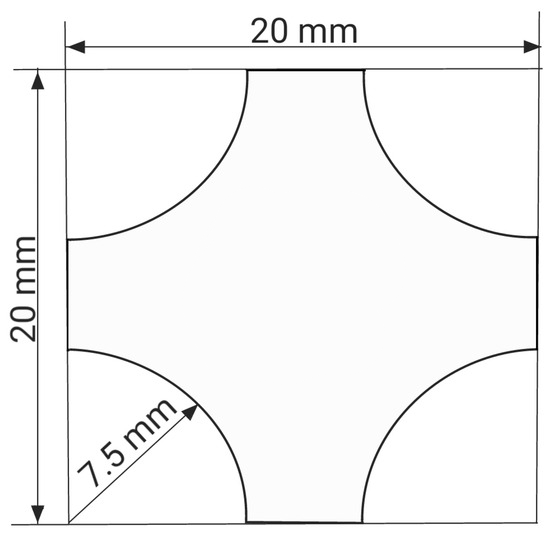
\includegraphics[width=0.4\textwidth]{../img/malt_geom.png}
  \caption{Geometry of the Maltese-cross specimen. The notch radius is identical for all cuts.}
  \label{fig:malt_geometry}
\end{figure}

\subsubsection{Data selection rules}
An observation window $\mathcal W_w\subset\Omega_0$ is defined around the geometric center and aligned with the mesh axes: a single central triangle (1-element), a $5\,\times\,5$ mm square, a $10\,\times\,10$ mm square, or the full field. At each load step $n=1,\dots,N$ and for each triangle $T$ with barycenter in $\mathcal W_w$, we record the pair $(\mathbb C_T^{(n)},\,\mathbb S_T^{(n)})$. Units: window sizes in mm; $\mathbb C$ dimensionless; $\mathbb S$ in MPa. Typical counts of elements in the observation window: 1 (1-element), 252 ($5\,\times\,5$ mm), 954 ($10\,\times\,10$ mm), and 5404 (full field).

\paragraph{Training/validation splits.}
For fixed protocol $p$ and window $w$, the base dataset $D(p,w)$ is split into training $D_{\mathrm{tr}}(p,w)$ and validation $D_{\mathrm{val}}(p,w)$. Because data collected from the central element yield axial components orders of magnitude larger than shear, expanding $w$ improves shear observability and reduces shear-prediction errors downstream.

\begin{figure}[H]
  \centering
  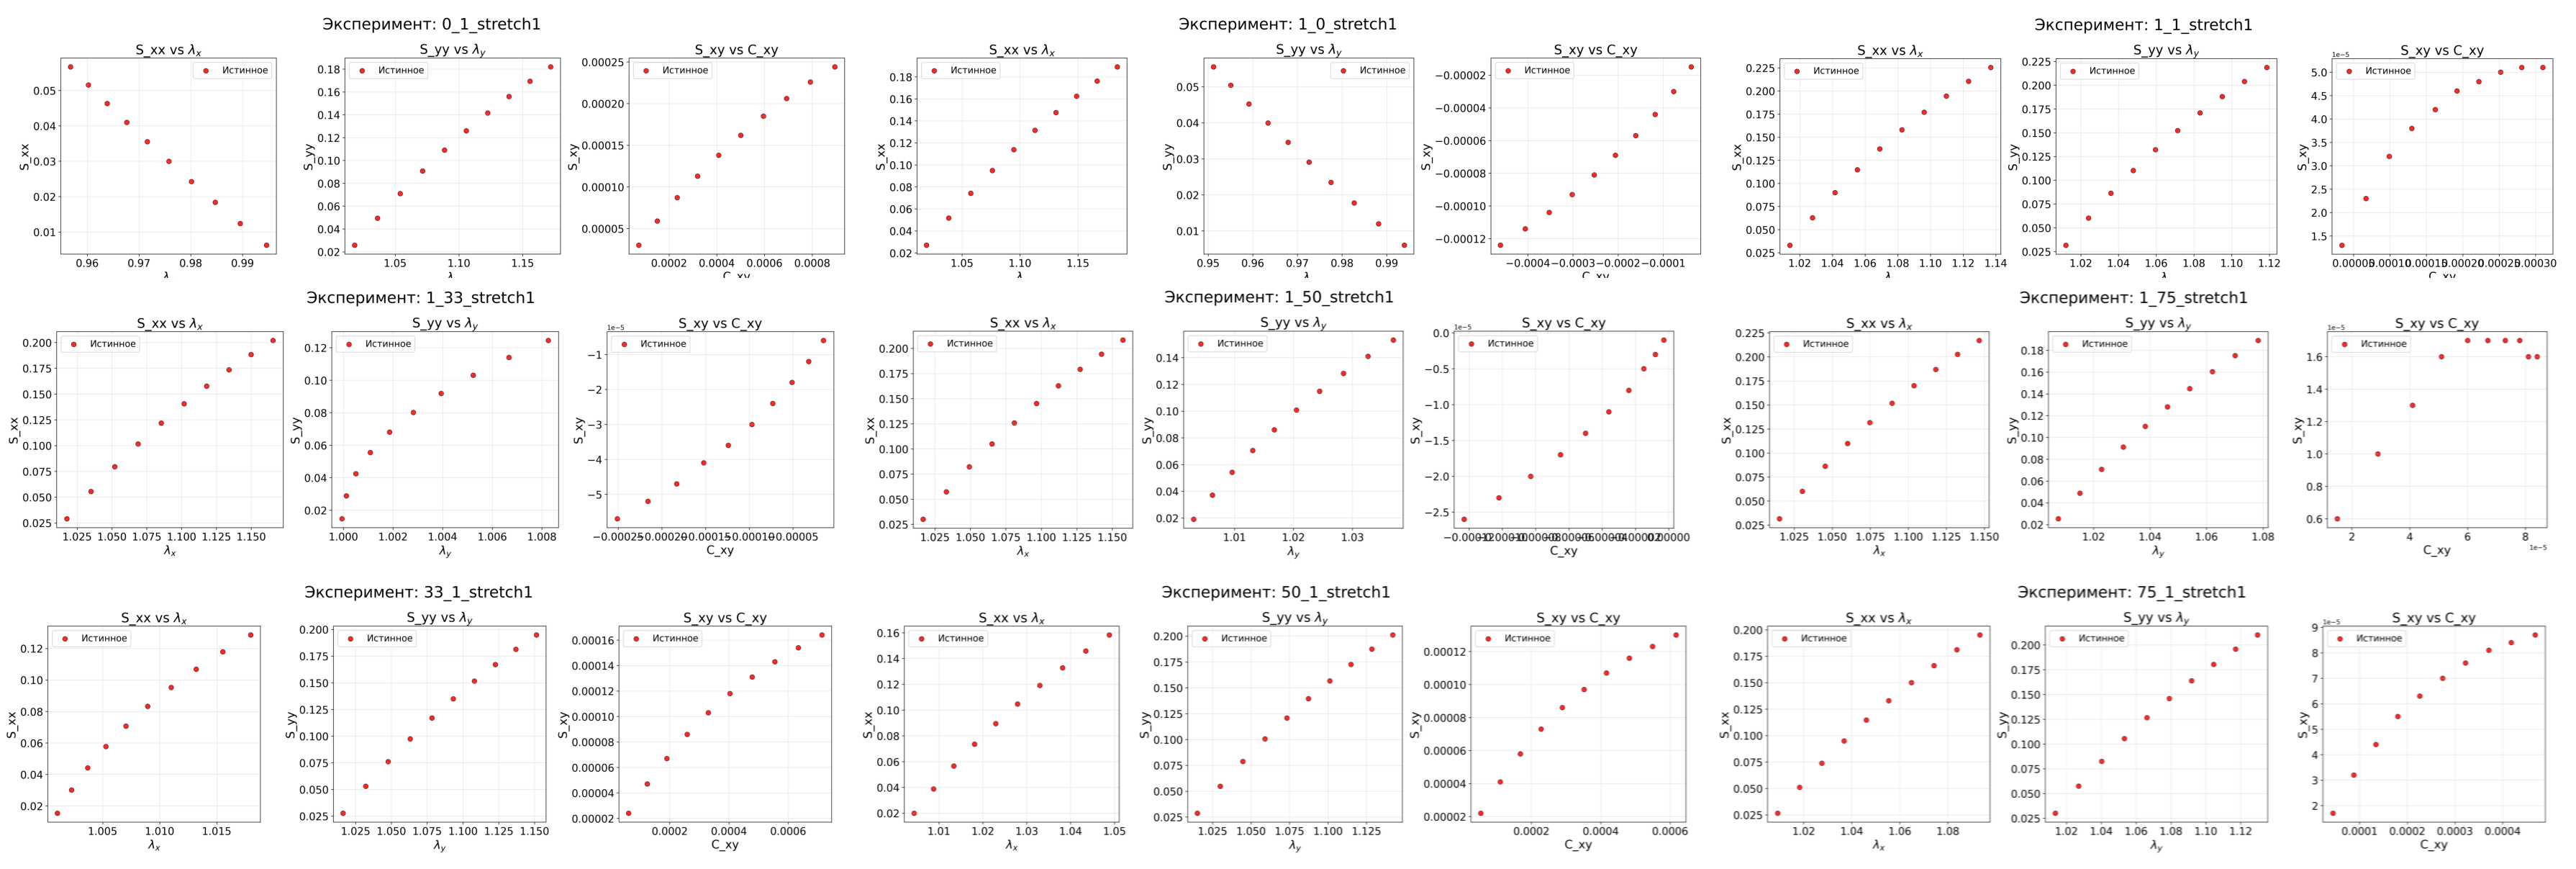
\includegraphics[width=1.0\textwidth]{../img/all_stress_plots.png}
  \caption{Example training dataset: stress components across load steps and protocols.}
  \label{fig:training_data}
\end{figure}

%%%%%%%%%%%%%%%%%%%%%%%%%%%%%%%%%%%%%%%%%%
% (Results section removed; content below belongs to Virtual Experiment)

% (Thermodynamic Consistency and Numerical Aspects paragraphs moved to earlier sections)

\subsection{Interpolation and Extrapolation of Loading Curves}
On biaxial loading of the Maltese-cross specimen, CLANN accurately interpolates and extrapolates axial stress components across load paths using small training subsets; shear components require richer data due to their small magnitudes in central regions. For quantitative evaluation we use: (i) the coefficient of determination $R^2$,
\begin{equation}\label{eq:r_squared_eng}
  R^2 = 1 - \frac{\sum_{i=1}^n (y_i - \hat{y}_i)^2}{\sum_{i=1}^n (y_i - \bar{y})^2},
\end{equation}
(ii) the pointwise relative error,
\begin{equation}\label{eq:rel_error_eng}
  \epsilon = \frac{\| \, \mathbb S - \mathbb S_{\text{ref}} \, \|}{\| \, \mathbb S_{\text{ref}} \, \|},
\end{equation}
and (iii) the P1-error combining absolute and relative contributions,
\begin{equation}\label{eq:p1_error_eng}
  \epsilon_{\mathrm{P1}} = \frac{\| \, \mathbb S - \mathbb S_{\text{ref}} \, \|}{s_0 + \| \, \mathbb S_{\text{ref}} \, \|},\qquad s_0 = \max(\mathbb S_{\text{pred}}).
\end{equation}
The following integral metrics (Frobenius norm) are also used on cell data: the absolute $L^2$-error,
\begin{equation}\label{eq:l2_abs_stress_cell_eng}
  \|e\|_{L^2} = \Bigg( \sum_{K} \| \, \mathbb S_{\text{ref},K} - \mathbb S_{\text{pred},K} \, \|_F^{2}\, |K| \Bigg)^{\tfrac12},
\end{equation}
and the relative $L^2$-error,
\begin{equation}\label{eq:l2_rel_stress_eng}
  \|e\|_{L^2,\,\mathrm{rel}}\;=\; \frac{\Big( \sum\limits_{K} 
  \| \, \mathbb S_{\mathrm{ref},K} - \mathbb S_{\mathrm{pred},K} \, \|_F^{2}\, |K| \Big)^{\tfrac12}}
  {\Big( \sum\limits_{K} \| \, \mathbb S_{\mathrm{ref},K} \, \|_F^{2}\, |K| \Big)^{\tfrac12}}\,.
\end{equation}
Representative curves are shown in Figure~\ref{fig:interp_extrap}.

\begin{figure}[H]
  \centering
  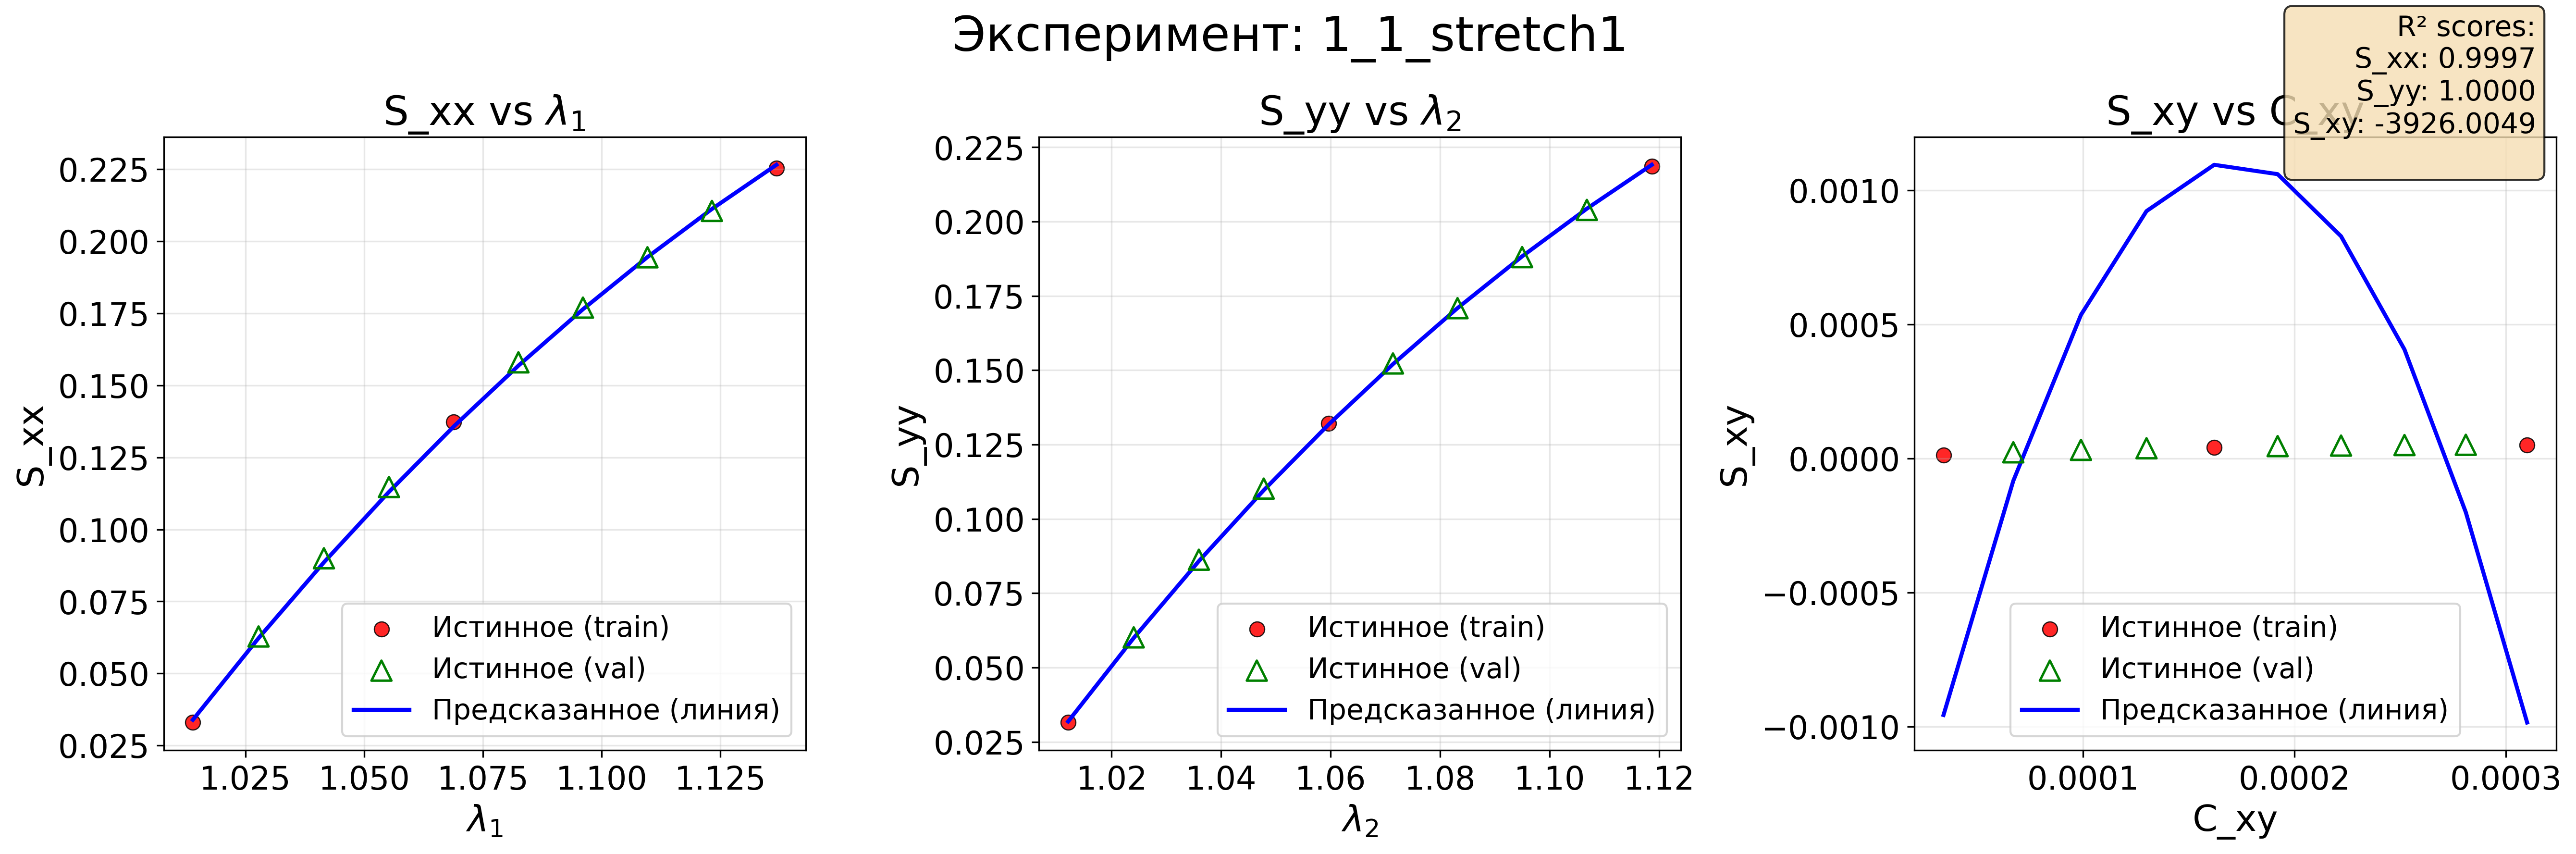
\includegraphics[width=0.48\textwidth]{../img/interpolation.png}\hfill
  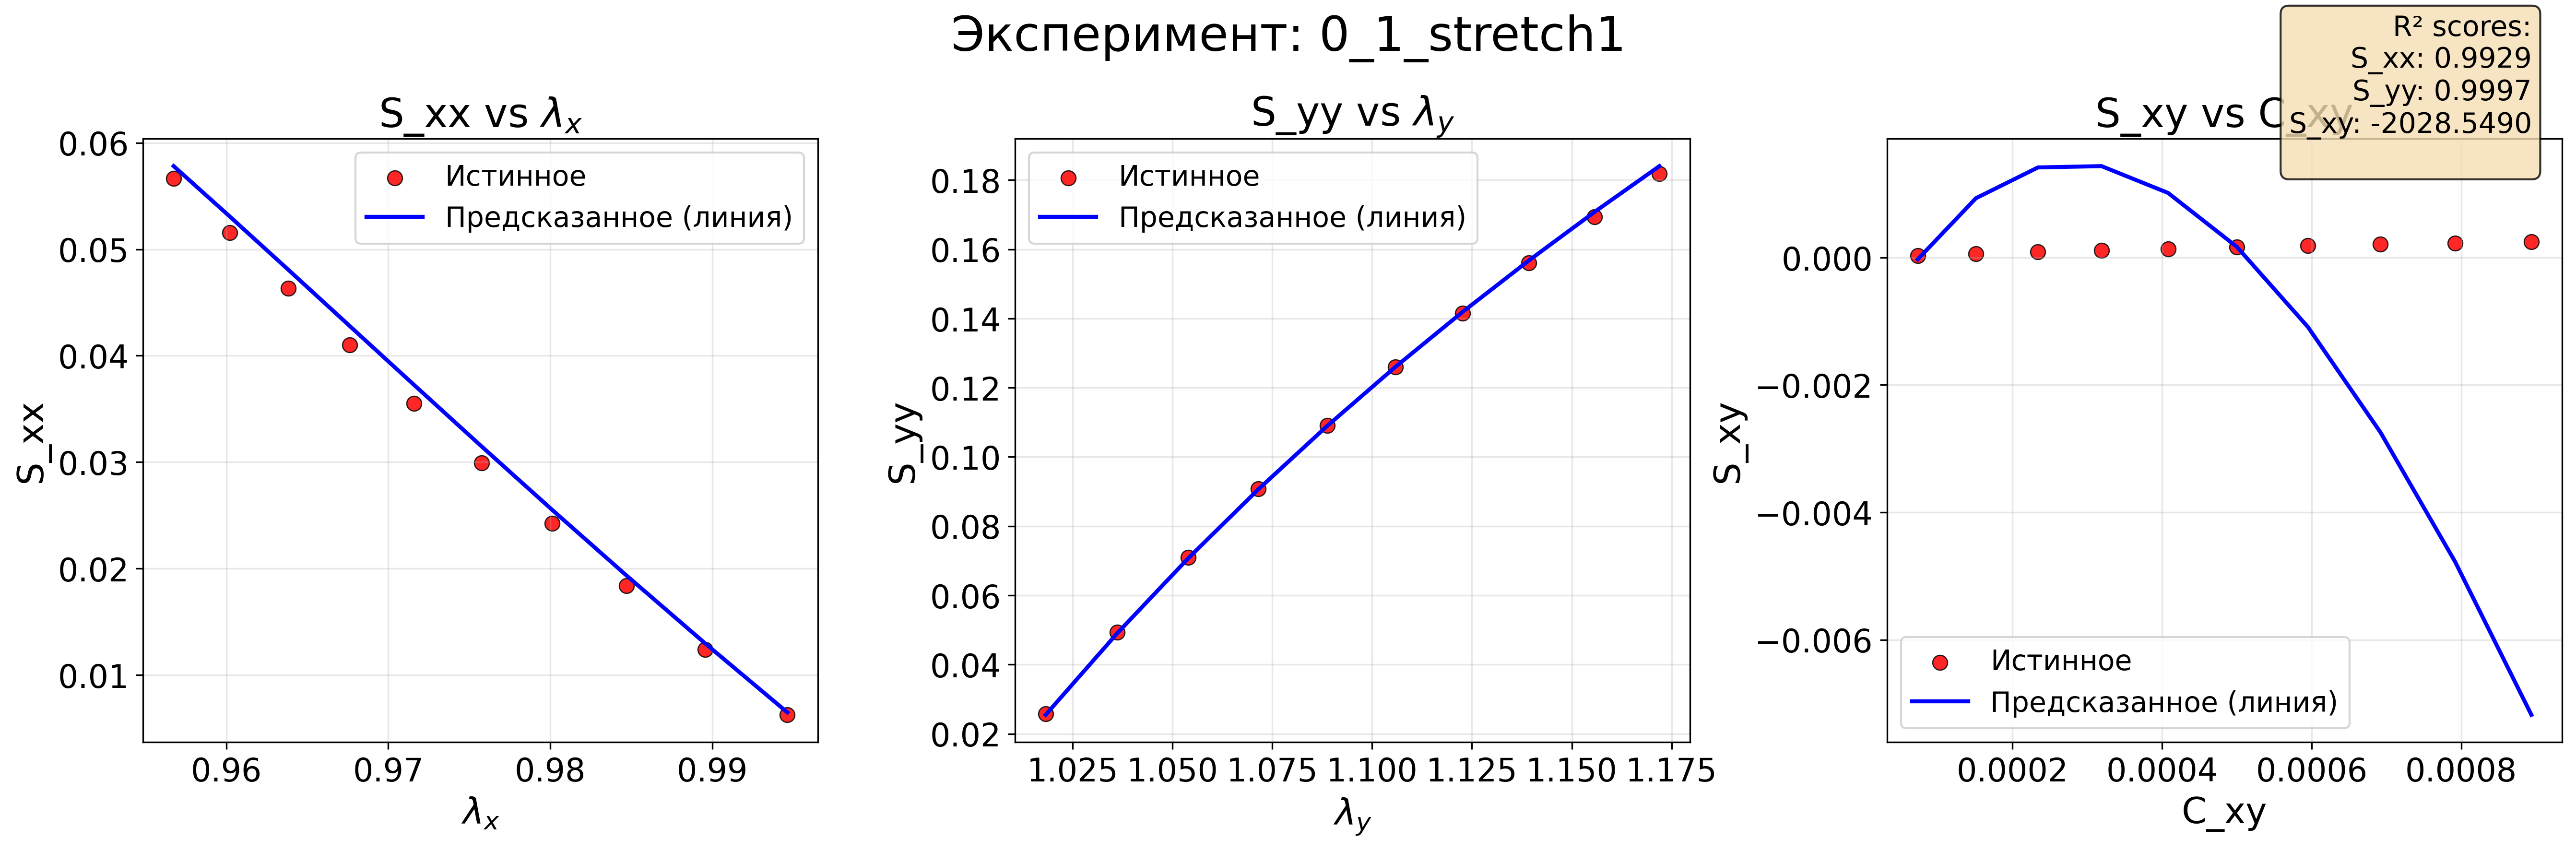
\includegraphics[width=0.48\textwidth]{../img/extrapolation.png}
  \caption{Interpolation (left) and extrapolation (right) of loading curves for selected protocols.}
  \label{fig:interp_extrap}
\end{figure}

\subsection{Membrane Inflation}
We evaluate CLANN in inflation of a clamped circular membrane ($R=25$ mm) under uniform pressure for (i) homogeneous thickness $T=0.54$ mm and (ii) heterogeneous thickness with two thickened sectors. Predicted PK2 stress fields agree with the reference hyperelastic solution for normal components; shear errors reduce as the observation window used for training increases, reflecting improved shear coverage.

\begin{figure}[H]
  \centering
  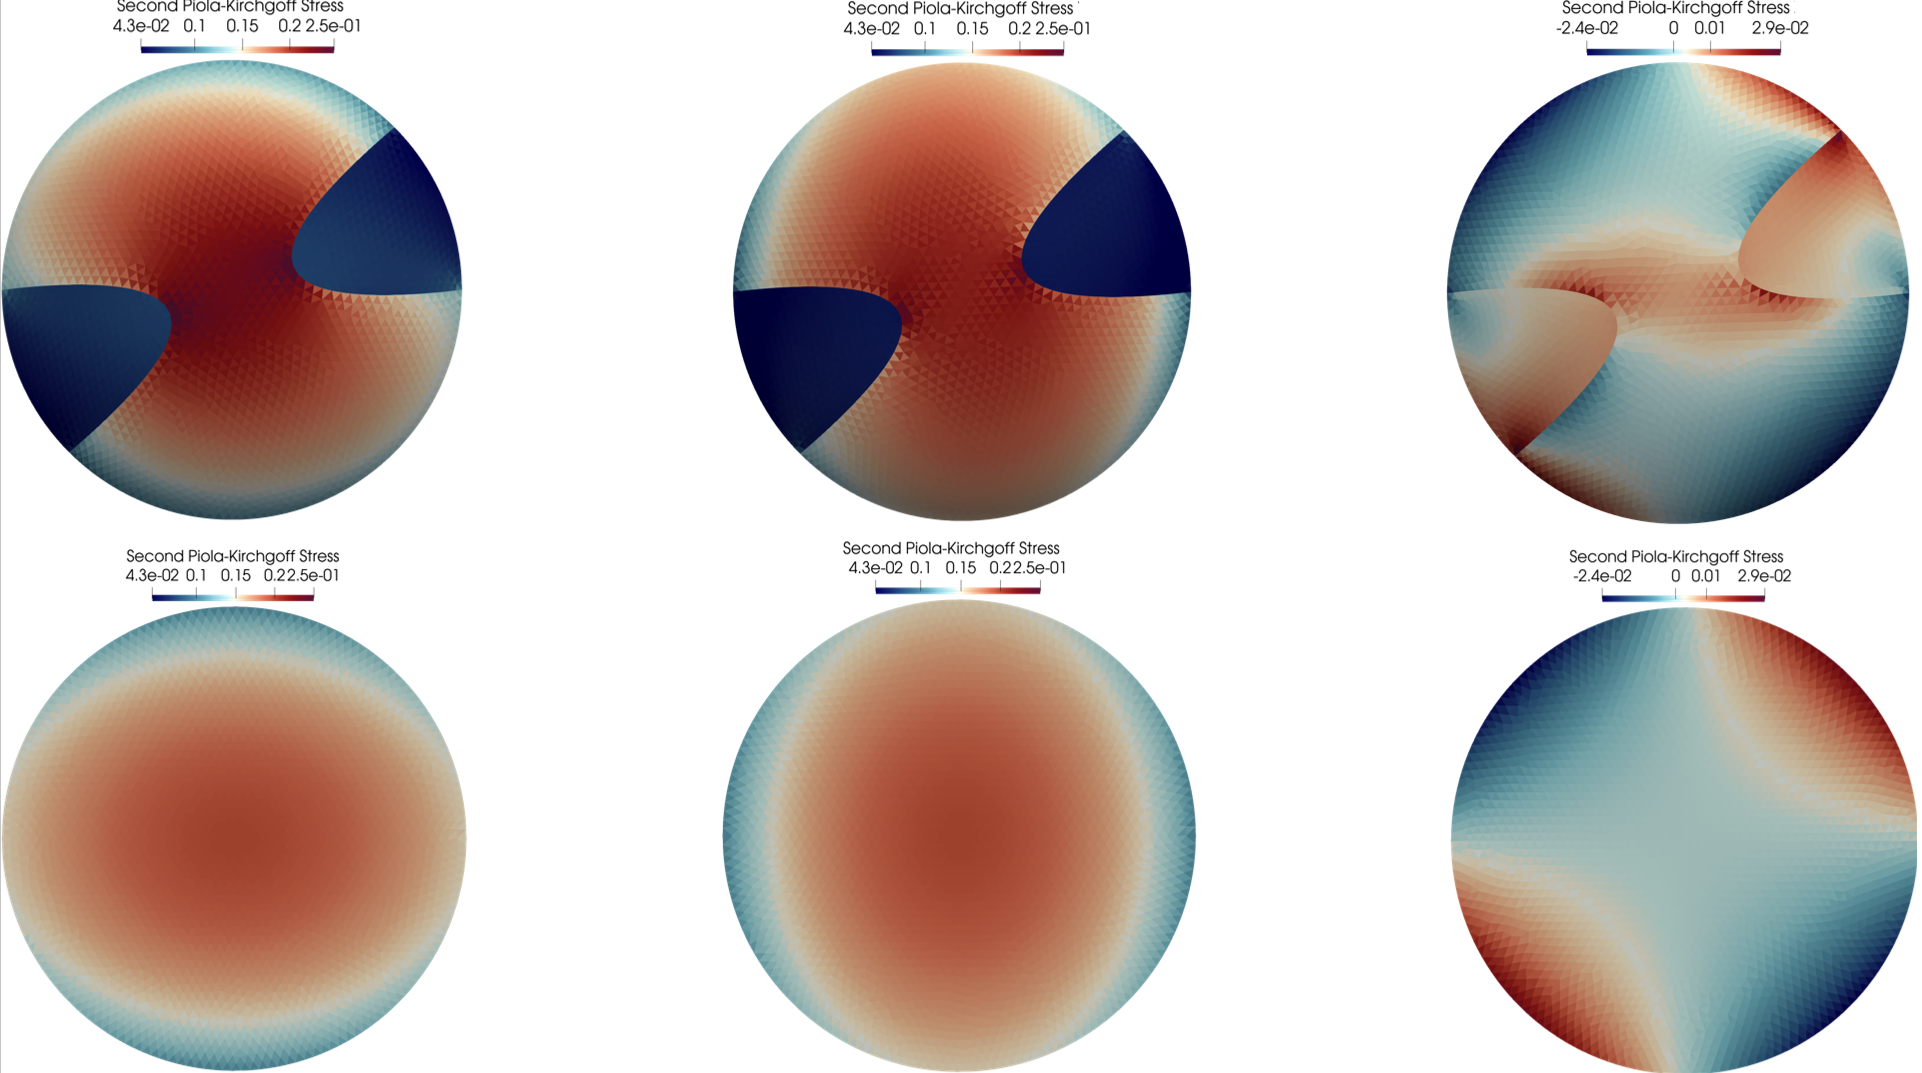
\includegraphics[width=0.6\textwidth]{../img/Numerical/ref_stress.png}
  \caption{Reference PK2 stress field in the inflated membrane (example).}
  \label{fig:inflation_ref}
\end{figure}

\begin{figure}[H]
  \centering
  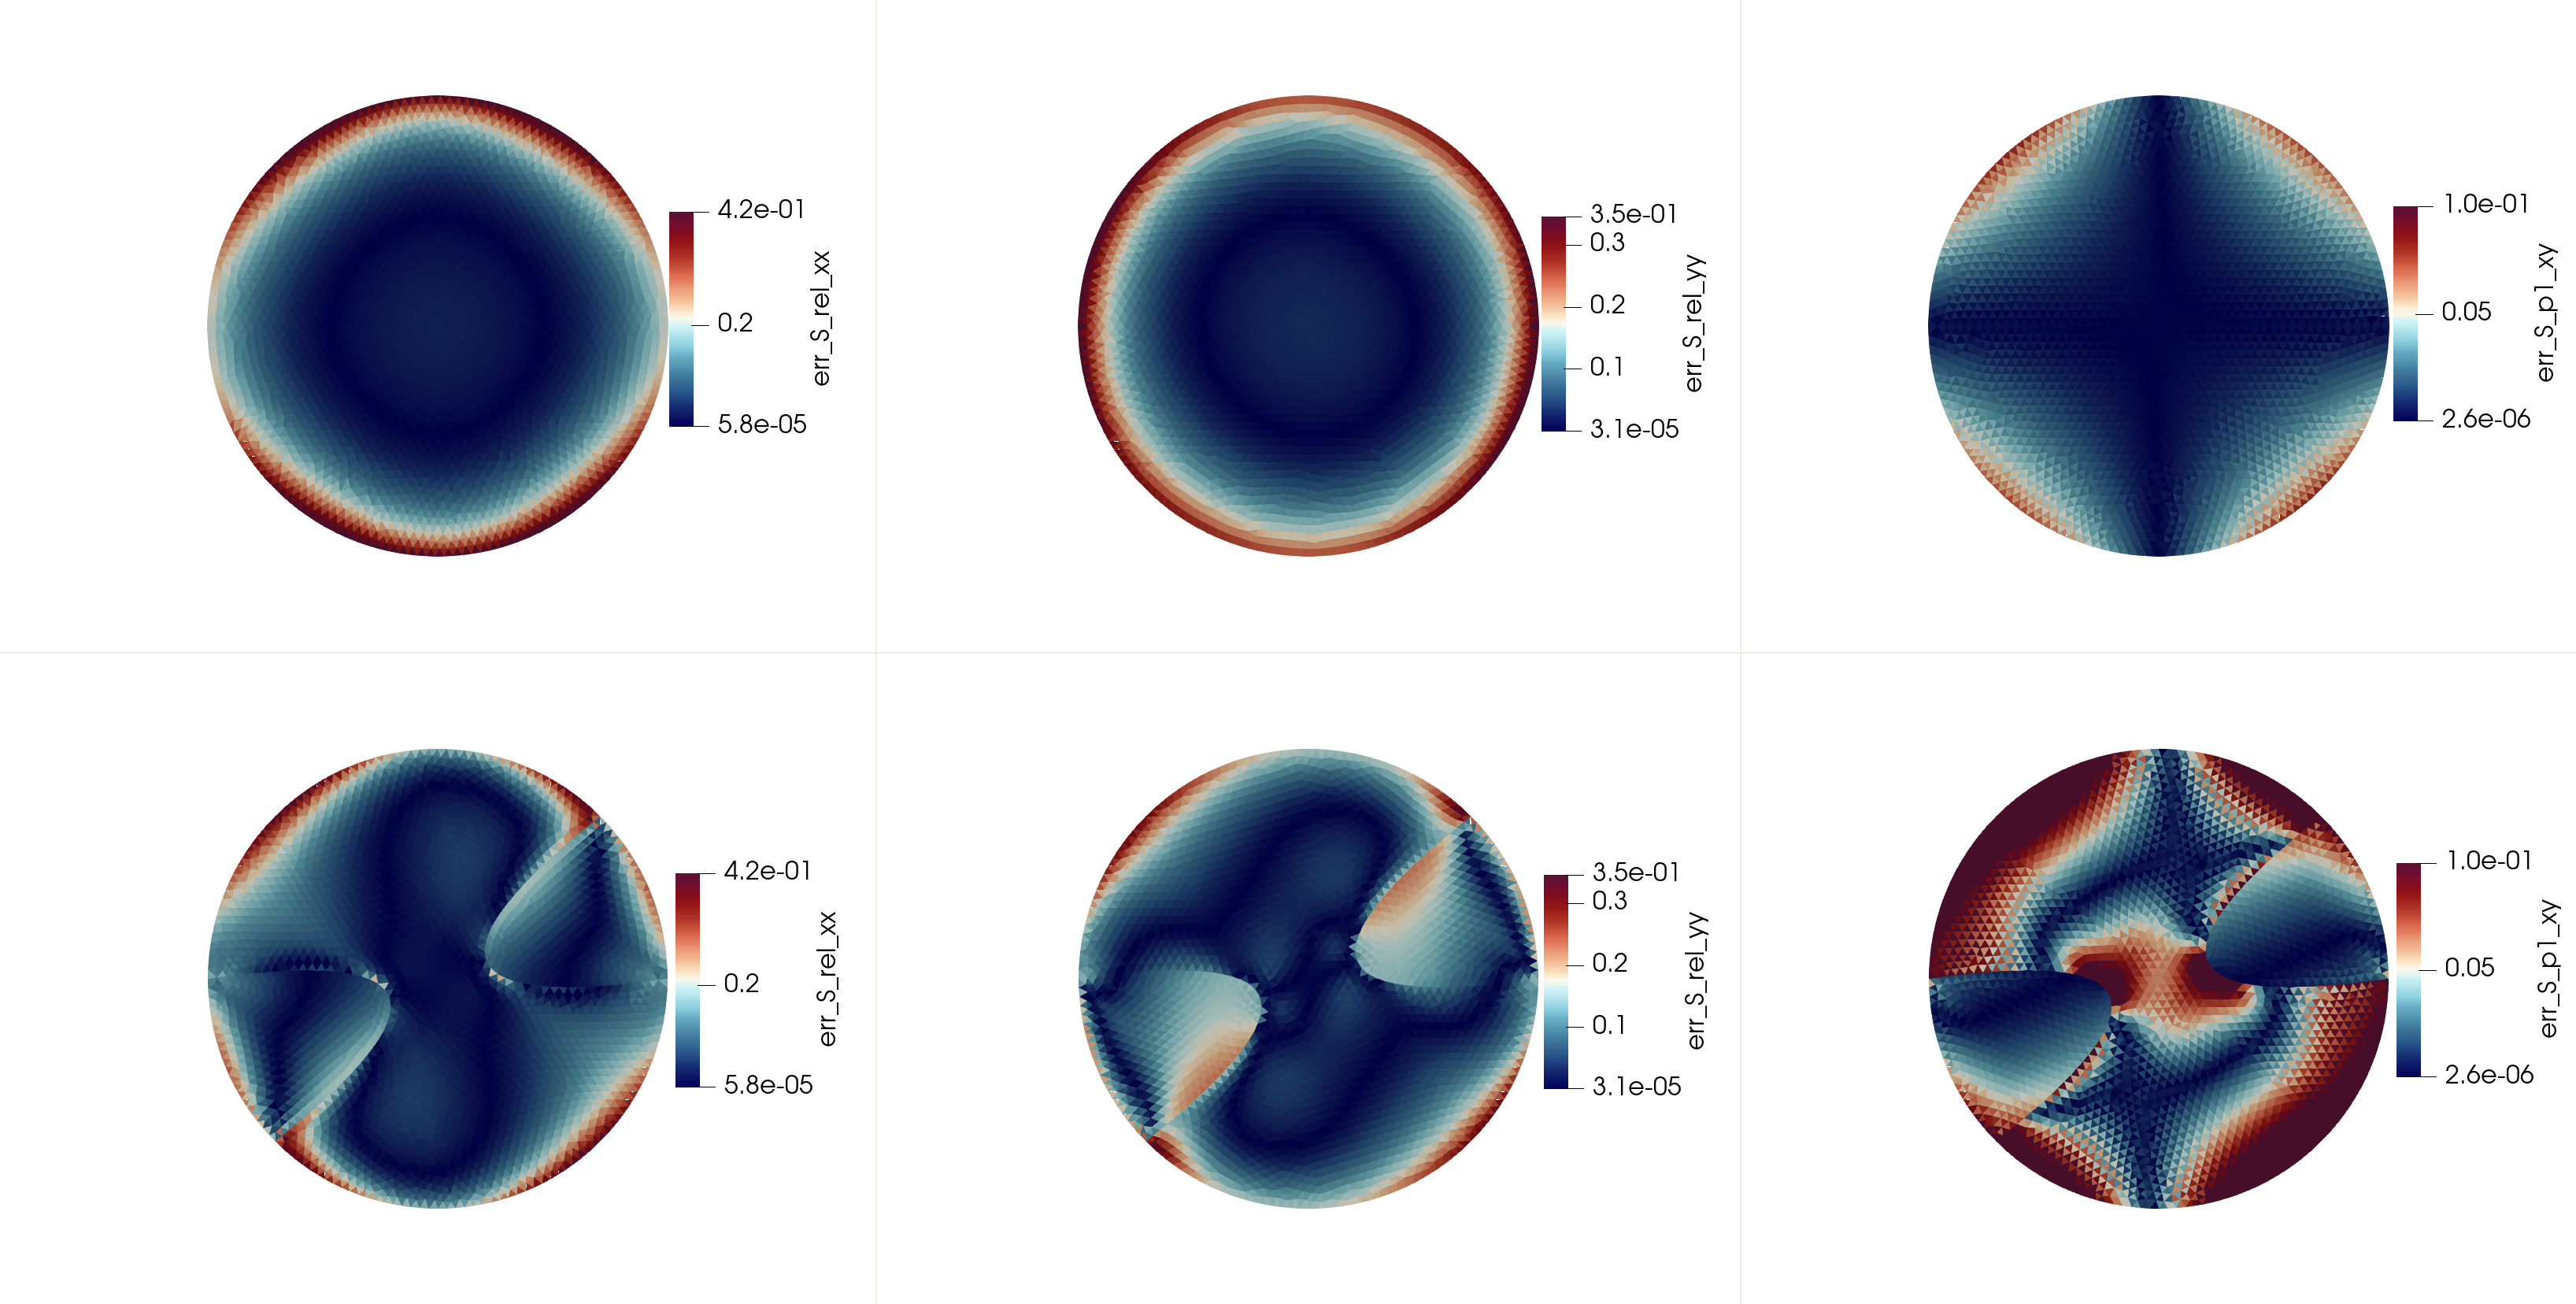
\includegraphics[width=0.9\textwidth]{../img/Numerical/errs.png}
  \caption{Error fields between predicted and reference stresses for representative cases.}
  \label{fig:inflation_errs}
\end{figure}

\begin{figure}[H]
  \centering
  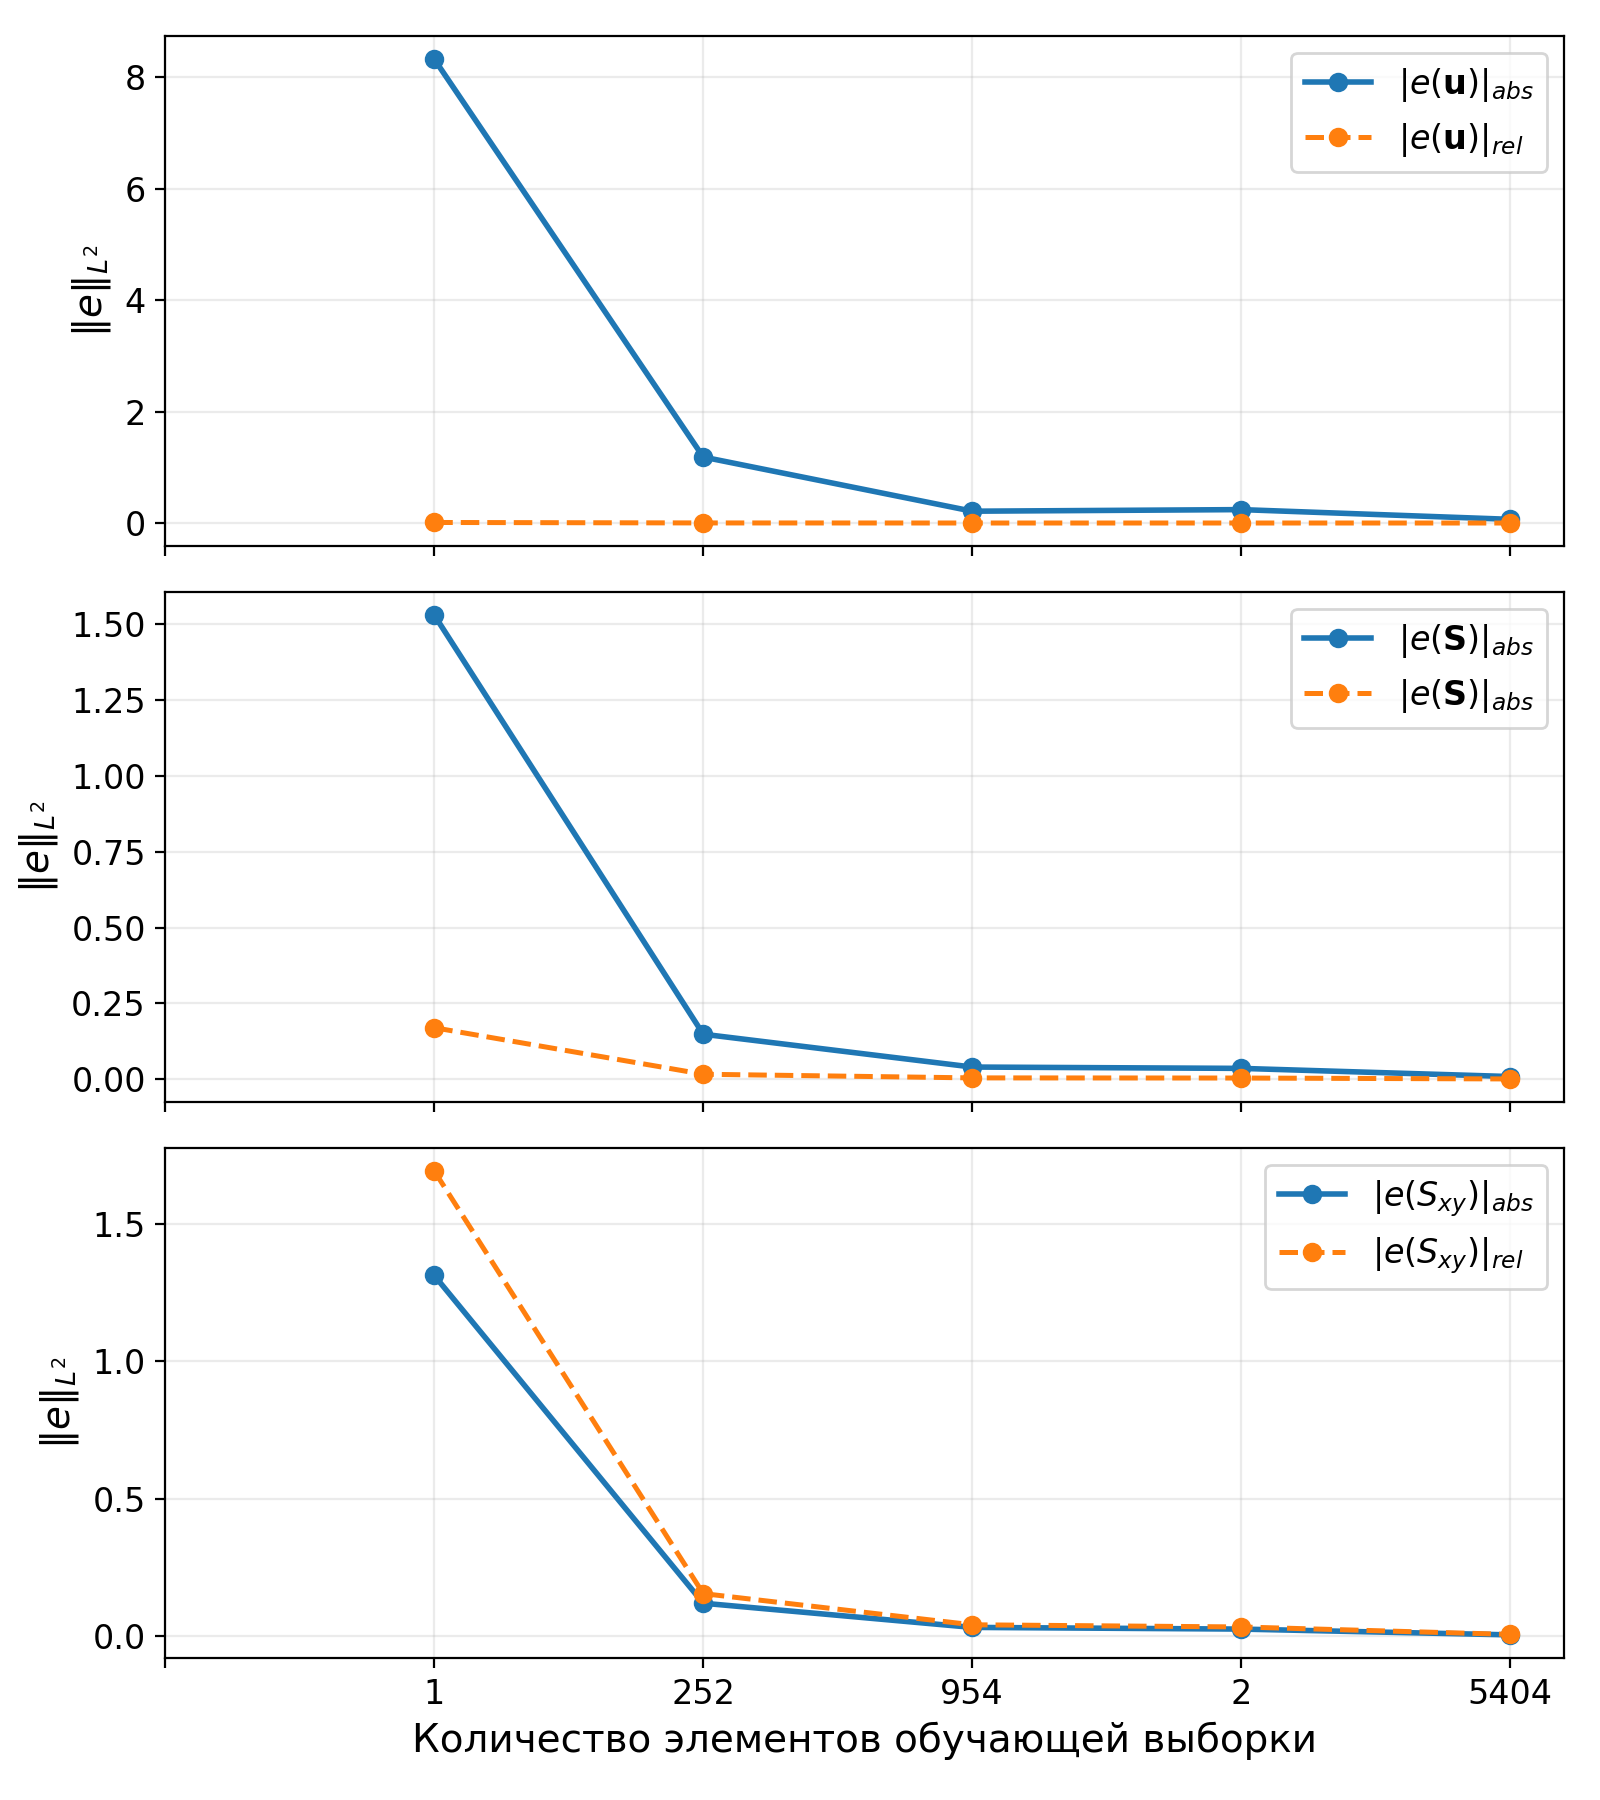
\includegraphics[width=0.5\textwidth]{../img/integral_errors.png}
  \caption{Integral stress errors vs. observation window size used for training.}
  \label{fig:integral_errors}
\end{figure}

\subsection{Computational Efficiency}
Due to convexity and availability of analytic Hessians, CLANN enables robust Newton-type solvers with predictable convergence. In our setup, CLANN outperforms local, table-driven data-driven baselines (e.g., kNN/IDW over Laplace strain space) by avoiding repeated nearest-neighbor queries and projection steps, while remaining competitive with classical hyperelastic forms in iteration counts. Runtime is primarily impacted by the efficiency of the model–solver interface.

\begin{table}[H]
\centering
\caption{Runtime (s) on membrane inflation: homogeneous vs. heterogeneous thickness}
\label{tab:experiments_summary_eng}
\begin{tabular}{|l|c|c|}
\hline
\textbf{Method} & \textbf{Homogeneous} & \textbf{Heterogeneous} \\
\hline
CLANN & 512 & 329 \\
\hline
Neo-Hooke & 13 & 16 \\
\hline
kNN & 993 & -- \\
\hline
\end{tabular}
\end{table}

%%%%%%%%%%%%%%%%%%%%%%%%%%%%%%%%%%%%%%%%%%
\section{Discussion}

CLANN unifies classical hyperelastic modeling with modern convex neural networks. Compared to traditional forms (Neo-Hookean, Mooney--Rivlin, Ogden), CLANN maintains the fundamental relationship \(S=\partial\psi/\partial C\) while learning \(\psi\) from data under strict convexity constraints. This yields improved stability and expressiveness, and it facilitates incorporation of priors such as near-incompressibility or anisotropy via extensions of the parameterization and network architecture. The convex design reduces non-physical responses and mitigates bifurcations in challenging loading paths.

%%%%%%%%%%%%%%%%%%%%%%%%%%%%%%%%%%%%%%%%%%
\section{Conclusions}

We introduced a mathematically grounded, thermodynamically consistent neural constitutive model for hyperelasticity. A Cholesky-based logarithmic parameterization and an ICNN energy ensure strict convexity, objective stresses, and positive-definite tangents. Explicit stress and Hessian formulas support efficient FE integration and robust Newton convergence. The framework recovers linear elasticity at small strains and is well-suited to soft-tissue biomechanics; future work will address anisotropy and near-incompressibility.

%%%%%%%%%%%%%%%%%%%%%%%%%%%%%%%%%%%%%%%%%%
\section{Patents}

Not applicable.

%%%%%%%%%%%%%%%%%%%%%%%%%%%%%%%%%%%%%%%%%%
\vspace{6pt} 

%%%%%%%%%%%%%%%%%%%%%%%%%%%%%%%%%%%%%%%%%%
%% optional
%\supplementary{The following supporting information can be downloaded at:  \linksupplementary{s1}, Figure S1: title; Table S1: title; Video S1: title.}

% Only for journal Methods and Protocols:
% If you wish to submit a video article, please do so with any other supplementary material.
% \supplementary{The following supporting information can be downloaded at: \linksupplementary{s1}, Figure S1: title; Table S1: title; Video S1: title. A supporting video article is available at doi: link.}

% Only used for preprtints:
% \supplementary{The following supporting information can be downloaded at the website of this paper posted on \href{https://www.preprints.org/}{Preprints.org}.}

% Only for journal Hardware:
% If you wish to submit a video article, please do so with any other supplementary material.
% \supplementary{The following supporting information can be downloaded at: \linksupplementary{s1}, Figure S1: title; Table S1: title; Video S1: title.\vspace{6pt}\\
%\begin{tabularx}{\textwidth}{lll}
%\toprule
%\textbf{Name} & \textbf{Type} & \textbf{Description} \\
%\midrule
%S1 & Python script (.py) & Script of python source code used in XX \\
%S2 & Text (.txt) & Script of modelling code used to make Figure X \\
%S3 & Text (.txt) & Raw data from experiment X \\
%S4 & Video (.mp4) & Video demonstrating the hardware in use \\
%... & ... & ... \\
%\bottomrule
%\end{tabularx}
%}

%%%%%%%%%%%%%%%%%%%%%%%%%%%%%%%%%%%%%%%%%%
\authorcontributions{The author solely developed the mathematical formulation and analysis of CLANN, drafted and revised the manuscript, and approved the published version.}

\funding{This research received no external funding.}

\institutionalreview{Not applicable.}

\informedconsent{Not applicable.}

\dataavailability{No new data were created or analyzed in this study.}

\acknowledgments{The author thanks colleagues for discussions that helped refine the mathematical presentation of CLANN.}

\conflictsofinterest{The author declares no conflict of interest.}

%%%%%%%%%%%%%%%%%%%%%%%%%%%%%%%%%%%%%%%%%%
%% Optional

%% Only for journal Encyclopedia
%\entrylink{The Link to this entry published on the encyclopedia platform.}

\abbreviations{Abbreviations}{
The following abbreviations are used in this manuscript:
\\

\noindent 
\begin{tabular}{@{}ll}
CLANN & Convex Laplace Artificial Neural Network\\
ICNN & Input Convex Neural Network\\
FE & Finite Element\\
SPD & Symmetric Positive Definite\\
PK2 & Second Piola--Kirchhoff (stress)\\
\end{tabular}
}

%%%%%%%%%%%%%%%%%%%%%%%%%%%%%%%%%%%%%%%%%%
%% Optional
\appendixtitles{yes}
\appendixstart
\appendix
\section{Equivalence of QR factorization of F and Cholesky of C=F$^{\top}$F for computing xi}
\label{app:cholesky}

\subsection{Setting and notation}
We consider two-dimensional hyperelastic kinematics. Let $\vect F\in\mathbb R^{2\times 2}$ with $\det\vect F>0$, $\vect C=\vect F^{\top}\vect F$ (SPD), and the Cholesky factorization $\vect C=\tilde{\vect F}^{\top}\tilde{\vect F}$ with $\tilde{\vect F}$ upper triangular and $\operatorname{diag}(\tilde{\vect F})>0$. Define the logarithmic coordinates $\boldsymbol{\xi}=(\ln u_{11},\ln u_{22}, u_{12}/u_{11})$ for $\tilde{\vect F}=[u_{ij}]$.

\subsection{Theorem (equivalence of $\vect U$ and $\vect R$)}
Let $\vect F\in\mathbb R^{2\times 2}$ be nonsingular with thin QR factorization $\vect F=\vect Q\vect R$, where $\vect Q$ is orthogonal and $\vect R$ is upper triangular with positive diagonal. Then $\vect R$ coincides with the Cholesky factor of $\vect C$:
\begin{equation}
\vect R = \operatorname{chol}(\vect C),\qquad \vect C=\vect F^{\top}\vect F.
\end{equation}
Proof: $\vect C=\vect F^{\top}\vect F=(\vect Q\vect R)^{\top}(\vect Q\vect R)=\vect R^{\top}\vect R$. Since $\vect C$ is SPD and $\vect R$ is upper triangular with positive diagonal, the representation $\vect C=\vect R^{\top}\vect R$ is unique, hence $\vect R=\operatorname{chol}(\vect C)$.

\subsection{Coordinates $\boldsymbol{\xi}$ via $\tilde{\vect F}$}
For $\tilde{\vect F}=\begin{bmatrix} \tilde f_{11} & \tilde f_{12} \\ 0 & \tilde f_{22} \end{bmatrix}$ with $\operatorname{diag}(\tilde{\vect F})>0$,
\begin{equation}
\boldsymbol{\xi}=(\xi_1,\xi_2,\xi_3)=(\ln\tilde f_{11}, \ln\tilde f_{22}, \tilde f_{12}/\tilde f_{11}).
\end{equation}

%%%%%%%%%%%%%%%%%%%%%%%%%%%%%%%%%%%%%%%%%%
%\isPreprints{} % If the paper is ``preprints'', please uncomment this parenthesis.
%\printendnotes[custom] % Un-comment to print a list of endnotes

\reftitle{References}

% Please provide either the correct journal abbreviation (e.g. according to the “List of Title Word Abbreviations” http://www.issn.org/services/online-services/access-to-the-ltwa/) or the full name of the journal.
% Citations and References in Supplementary files are permitted provided that they also appear in the reference list here. 

%=====================================
% References, variant A: external bibliography
%=====================================
% \bibliography{your_external_BibTeX_file}

%=====================================
% References, variant B: internal bibliography
%=====================================

% ACS format
\isAPAandChicago{}{%
\begin{thebibliography}{999}
% Reference 1
\bibitem[Author1(year)]{ref-journal}
Author~1, T. The title of the cited article. {\em Journal Abbreviation} {\bf 2008}, {\em 10}, 142--149.
% Reference 2
\bibitem[Author2(year)]{ref-book1}
Author~2, L. The title of the cited contribution. In {\em The Book Title}; Editor 1, F., Editor 2, A., Eds.; Publishing House: City, Country, 2007; pp. 32--58.
% Reference 3
\bibitem[Author1 and Author2 (year)]{ref-book2}
Author 1, A.; Author 2, B. \textit{Book Title}, 3rd ed.; Publisher: Publisher Location, Country, 2008; pp. 154--196.
% Reference 4
\bibitem[Author4(year)]{ref-unpublish}
Author 1, A.B.; Author 2, C. Title of Unpublished Work. \textit{Abbreviated Journal Name} year, \textit{phrase indicating stage of publication (submitted; accepted; in press)}.
% Reference 5
\bibitem[Author8(year)]{ref-url}
Title of Site. Available online: URL (accessed on Day Month Year).
% Reference 6
\bibitem[Author6(year)]{ref-proceeding}
Author 1, A.B.; Author 2, C.D.; Author 3, E.F. Title of presentation. In Proceedings of the Name of the Conference, Location of Conference, Country, Date of Conference (Day Month Year); Abstract Number (optional), Pagination (optional).
% Reference 7
\bibitem[Author7(year)]{ref-thesis}
Author 1, A.B. Title of Thesis. Level of Thesis, Degree-Granting University, Location of University, Date of Completion.
\end{thebibliography}
}

% Chicago format (Used for journal: arts, genealogy, histories, humanities, jintelligence, laws, literature, religions, risks, socsci)
\isChicagoStyle{%
\begin{thebibliography}{999}
% Reference 1
\bibitem[Aranceta-Bartrina(1999a)]{ref-journal}
Aranceta-Bartrina, Javier. 1999a. Title of the cited article. \textit{Journal Title} 6: 100--10.
% Reference 2
\bibitem[Aranceta-Bartrina(1999b)]{ref-book1}
Aranceta-Bartrina, Javier. 1999b. Title of the chapter. In \textit{Book Title}, 2nd ed. Edited by Editor 1 and Editor 2. Publication place: Publisher, vol. 3, pp. 54–96.
% Reference 3
\bibitem[Baranwal and Munteanu {[1921]}(1955)]{ref-book2}
Baranwal, Ajay K., and Costea Munteanu. 1955. \textit{Book Title}. Publication place: Publisher, pp. 154--96. First published 1921 (op-tional).
% Reference 4
\bibitem[Berry and Smith(1999)]{ref-thesis}
Berry, Evan, and Amy M. Smith. 1999. Title of Thesis. Level of Thesis, Degree-Granting University, City, Country. Identifi-cation information (if available).
% Reference 5
\bibitem[Cojocaru et al.(1999)]{ref-unpublish}
Cojocaru, Ludmila, Dragos Constatin Sanda, and Eun Kyeong Yun. 1999. Title of Unpublished Work. \textit{Journal Title}, phrase indicating stage of publication.
% Reference 6
\bibitem[Driver et al.(2000)]{ref-proceeding}
Driver, John P., Steffen Rohrs, and Sean Meighoo. 2000. Title of Presentation. In \textit{Title of the Collected Work} (if available). Paper presented at Name of the Conference, Location of Conference, Date of Conference.
% Reference 7
\bibitem[Harwood(2008)]{ref-url}
Harwood, John. 2008. Title of the cited article. Available online: URL (accessed on Day Month Year).
\end{thebibliography}
}{}

% APA format (Used for journal: admsci, behavsci, businesses, econometrics, economies, education, ejihpe, games, humans, ijfs, journalmedia, jrfm, languages, psycholint, publications, tourismhosp, youth)
\isAPAStyle{%
\begin{thebibliography}{999}
% Reference 1
\bibitem[\protect\citeauthoryear{Azikiwe \BBA\ Bello}{{2020a}}]{ref-journal}
Azikiwe, H., \& Bello, A. (2020a). Title of the cited article. \textit{Journal Title}, \textit{Volume}(Issue), 
Firstpage--Lastpage/Article Number.
% Reference 2
\bibitem[\protect\citeauthoryear{Azikiwe \BBA\ Bello}{{2020b}}]{ref-book1}
Azikiwe, H., \& Bello, A. (2020b). \textit{Book title}. Publisher Name.
% Reference 3
\bibitem[Davison(1623/2019)]{ref-book2}
Davison, T. E. (2019). Title of the book chapter. In A. A. Editor (Ed.), \textit{Title of the book: Subtitle} 
(pp. Firstpage--Lastpage). Publisher Name. (Original work published 1623) (Optional).
% Reference 4
\bibitem[Fistek et al.(2017)]{ref-proceeding}
Fistek, A., Jester, E., \& Sonnenberg, K. (2017, Month Day). Title of contribution [Type of contribution]. Conference Name, Conference City, Conference Country.
% Reference 5
\bibitem[Hutcheson(2012)]{ref-thesis}
Hutcheson, V. H. (2012). \textit{Title of the thesis} [XX Thesis, Name of Institution Awarding the Degree].
% Reference 6
\bibitem[Lippincott \& Poindexter(2019)]{ref-unpublish}
Lippincott, T., \& Poindexter, E. K. (2019). \textit{Title of the unpublished manuscript} [Unpublished manuscript/Manuscript in prepara-tion/Manuscript submitted for publication]. Department Name, Institution Name.
% Reference 7
\bibitem[Harwood(2008)]{ref-url}
Harwood, J. (2008). \textit{Title of the cited article}. Available online: URL (accessed on Day Month Year).
\end{thebibliography}
}{}

% If authors have biography, please use the format below
%\section*{Short Biography of Authors}
%\bio
%{\raisebox{-0.35cm}{\includegraphics[width=3.5cm,height=5.3cm,clip,keepaspectratio]{Definitions/author1.pdf}}}
%{\textbf{Firstname Lastname} Biography of first author}
%
%\bio
%{\raisebox{-0.35cm}{\includegraphics[width=3.5cm,height=5.3cm,clip,keepaspectratio]{Definitions/author2.jpg}}}
%{\textbf{Firstname Lastname} Biography of second author}

% For the MDPI journals use author-date citation, please follow the formatting guidelines on http://www.mdpi.com/authors/references
% To cite two works by the same author: \citeauthor{ref-journal-1a} (\citeyear{ref-journal-1a}, \citeyear{ref-journal-1b}). This produces: Whittaker (1967, 1975)
% To cite two works by the same author with specific pages: \citeauthor{ref-journal-3a} (\citeyear{ref-journal-3a}, p. 328; \citeyear{ref-journal-3b}, p.475). This produces: Wong (1999, p. 328; 2000, p. 475)

%%%%%%%%%%%%%%%%%%%%%%%%%%%%%%%%%%%%%%%%%%
%% for journal Sci
%\reviewreports{\\
%Reviewer 1 comments and authors’ response\\
%Reviewer 2 comments and authors’ response\\
%Reviewer 3 comments and authors’ response
%}
%%%%%%%%%%%%%%%%%%%%%%%%%%%%%%%%%%%%%%%%%%
\PublishersNote{}
%\isPreprints{} % If the paper is ``preprints'', please uncomment this parenthesis.
\end{document}

